%
% Homework Details
% - Title
% - Due date
% - University
% - Class
% - Class Alias
% - Class Section
% - Instructor
% - Author
% - AuthorID
%

\newcommand{\hmwkID}{1}
\newcommand{\hmwkTitle}{Final Project Report}
\newcommand{\hmwkTopic}{Game Playing with DQfD and DQN}
\newcommand{\hmwkUniversity}{NTU}
\newcommand{\hmwkClass}{Applied Deep Learning}
\newcommand{\hmwkClassAlias}{ADL}
\newcommand{\hmwkClassSection}{Fall 2017}
\newcommand{\hmwkClassInstructor}{Yun-Nung (Vivian) Chen and Hung-Yi Lee}
\newcommand{\hmwkTeam}{Praise The Sun}
\newcommand{\langver}{English}



\documentclass{article}

%
% Packages
%

\usepackage{enumitem}
\usepackage{amsmath}
\usepackage{fancyhdr}
\usepackage{lastpage}
\usepackage{titlesec}
\usepackage[hidelinks]{hyperref}
\usepackage{cleveref}
\usepackage{listings}
\usepackage{bm}
\usepackage{float}
\usepackage{amsthm}
\usepackage{booktabs}

\usepackage{pgfplots}
\pgfplotsset{compat=1.7}
\usepackage{pgf,tikz}
\usepackage{mathrsfs}
\usetikzlibrary{arrows}
\usetikzlibrary[patterns]

\usepackage{xcolor}
\hypersetup{
    colorlinks,
    linkcolor={red!50!black},
    citecolor={blue!50!black},
    urlcolor={blue!80!black}
}

% additional packages
\usepackage{lettrine} % large initial
\usepackage{amsfonts} % mathbb

%
% Chinese
%

\usepackage{xeCJK}
\setCJKmainfont{Noto Sans CJK TC Regular}

\XeTeXlinebreaklocale "zh"
\XeTeXlinebreakskip = 0pt plus 1pt

%
% Basic Document Settings
%

\topmargin=-0.45in
\evensidemargin=0in
\oddsidemargin=0in
\textwidth=6.5in
\textheight=9.0in
\headsep=0.25in

\linespread{1.3}

% multirow
\usepackage{multirow}
\usepackage{multicol}
\usepackage{arydshln}
% figure name
%\renewcommand{\figurename}{圖}
%\renewcommand{\tablename}{表}

\makeatletter
\def\hlinewd#1{%
  \noalign{\ifnum0=`}\fi\hrule \@height #1 \futurelet
   \reserved@a\@xhline}
\makeatother

% fancy style

\pagestyle{fancy}
%\lhead{\hmwkTeam}
\lhead{\hmwkClass\ (\hmwkUniversity, \hmwkClassSection)}
%\chead{}
\rhead{\hmwkTeam: \hmwkTitle\ (\langver)}
%\rhead{\hmwkClass\ (\hmwkUniversity, \hmwkClassSection): \hmwkTitle (\langver)}
\cfoot{\thepage\ of \pageref{LastPage}}

%
% Title Page
%

%\title{
%  % \vspace{2in}
%  \textmd{\textbf{\hmwkClass:\ \hmwkTitle}}\\
%  \textmd{\textbf{\hmwkTopic}} \\
%  \vspace{0.1in}\large{\textit{Instructors \hmwkClassInstructor}}
%  % \vspace{3in}
%}

\title{
   \vspace{-1.5cm}
  \hmwkClass:\ \hmwkTitle\\
  \textbf{\hmwkTopic} \\
  \vspace{0.1in}\large{\textit{Instructors: \hmwkClassInstructor}}
   %\vspace{-1.5cm}
}

\author{
    \textit{Team: \textbf{\hmwkTeam}}
}
\date{}

\begin{document}

%\pagenumbering{gobble}
\maketitle
\thispagestyle{empty}
\thispagestyle{fancy}
% \pagebreak
\pagenumbering{arabic}

\lettrine[findent=1pt]{\fbox{D}}{ }eep reinforcement learning are learning models that combines traditional reinforcement learning algorithms with modern state-of-the-art deep learning models. Currently, many applications, such as robotics and game playing, have reached astonishing performances with these kinds of models. However, these models require huge amount of time/self-generated data to achieve favorable results. What worse is that the performances are sometimes even unstable: the results may differ even given the same environments and model settings. Some recent advanced algorithms may make the training process more efficient, for instance, the \emph{Deep Q-Learning from Demonstrations}(DQfD) proposed by (T. Hester et al., 2017)\cite{DBLP:journals/corr/HesterVPLSPSDOA17}, which introduced the so-called ``demonstration data'' that can train deep RL models in a supervised manner. In this project, we used some Atari games as the training environment, and we did some experiments on some traditional value-based deep reinforcement learning algorithms and on DQfD, and made some comparisons and analysis on our experiments.

\section{Background}
A reinforcement learning model contains an environment and an agent, in which the behavior of the agent can be modeled as a Markov decision process (MDP). MDP can be formally represented by a 5-tuple $(S,A,R(\cdot,\cdot),T(\cdot, \cdot, \cdot),\gamma)$, where $S$ denotes the set of states, $A$ represents the set of all possible actions, $R(s,a)$ is a reward function (given current state $s$ and action $a$, $R$ returns the reward), $T(s,a,s')=P(s'|s,a)$ is a transition function, which follows some distribution, and $\gamma$ is the discount factor. The agent can be regarded as being applying some policy function $\pi(s)$ in the environment to take actions.\par

The most common reinforcement learning models can be classified as \emph{policy-baced} and \emph{value-based}. The former tries to find a policy function $\pi$ such that it can be as close with the optimal policy as possible (i.e. $\pi \rightarrow \pi^*$), while the latter is to learn a value function $Q^\pi (s,a)$, whose objective is to estimate the expected value given the current state $s$ and action $a$, and we hope that the value function we are training can be as close to the optimal one as possible (i.e. $Q^\pi (s,a) \rightarrow Q^* (s,a)$). Under such circumstance, the optimal policy for the agent will be $\pi^*(s) = \arg \underset{a \in A}\max\ Q^*(s,a)$.\par

Deep Q Learning (DQN) is one of the most common value-based deep learning algorithms. Its optimal value function can be represented as a Bellman equation:
\[Q^*(s,a) = \mathbb{E}\left[R(s,a) + \gamma \sum_{s'}P(s'|s,a) \underset{a'}\max\ Q^*(s',a')\right]\]
In a DQN model, we'll use a neural network to represent $Q^\pi$,and we expect that $Q^\pi$ will eventually converge to $Q^*$. In practice, we often use mean squared error (MSE) as the loss function for training, and moreover, for stablility, we also stablize the weights of the target network, and the loss function is as follows:
\[\mathcal{L}(w) = \mathbb{E}\left[\left(\underbrace{R(s,a) + \gamma \underset{a'}\max\ Q(s',a', w^-)}_{\text{target, update slowly}} - \underbrace{Q(s,a,w)}_{\text{online, update quickly}}\right)^2\right]\]
\par
There are some other common DQN models, including Double Q-Learning(DDQN)(H. van Hasselt et al., 2015)\cite{DBLP:journals/corr/HasseltGS15}, Dueling Network (Z. Wang et al., 2015)\cite{DBLP:journals/corr/WangFL15}, etc. The former points out that upward bias may occurs when using target network to select the action that has the largest expected value, and thus the (new) loss function is as follows:
\[\mathcal{L}(w) = \mathbb{E}\left[\left(R(s,a) + \gamma Q(s',\underbrace{\arg \underset{a'}\max\ Q(s',a',w)}_{\text{online network chooses optimal } a'}, w^-) - Q(s,a,w)\right)^2\right]\], while the latter modifies the network as:
\[Q(s,a,w) = \underbrace{V(s,w)}_{\text{\emph{value}, action-independent}} + \underbrace{A(s,a,w)}_{\text{\emph{advantage}, action-dependent}}\]
The basic idea is that some states are just better (regardless of the actions taken), while others not. Hence the expected value can be cosidered to be the sum of the expected value of the state (action-independent) and the added/subtracted value given a certain action.


\section{DQfD:Learning from Demonstrated Data}


DQfD is a kind of deep reinforcement learning algorithm that contains elements of supervised learning. Unlike the original DQN, DQfD will perform pre-training on some pre-collected demonstration data prior to the real reinforcement learning process. One can imagine that the agent is similar to an athlete, and the athlete will first train his/her skills from a couch (i.e. expert's demonstration), and then accumulate his/her experiences in matches (i.e. environment), but not taking part in matches in the very beginning. Besides, the loss function of DQfD are also different. First, we must make sure that the model does learn the actions of the demonstrator, so we add the supervised loss, which is shown as follows:
\[\mathcal{L}_E(w) = \underset{a \in A}\max [Q(s,a,w) + l(a_E, a)] - Q(s, a_E)\text{, where }l(a_E, a) = \left\{\begin{array}{cl}0 & \text{, if } a = a_E\\ k & \text{, otherwise and } k \text{ is a positive number}\end{array}\right.\]
This will force the expected values of all the other actions to become at least a margin (k) lower than the value of $a_E$, such that the model will have more tendency to learn the actions from demonstrated data. Other than that, we also impose an L2-regularization loss ($\mathcal{L}_{L2}(w)$)on network weights and bias so as to prevent overfitting on demonstrated data. Finally, according to the original paper, in order to satisfy the Bellman equation, an n-step loss ($\mathcal{L}_n(w)$) is also computed. The total loss is:
\[\mathcal{L}(w) = \underbrace{\mathcal{L}_{DQ}(w)}_{\text{original loss}} + \lambda_n \underbrace{\mathcal{L}_{n}(w)}_{\text{n-step loss}} + \lambda_E \underbrace{\mathcal{L}_{E}(w)}_{\text{supervised loss}} + \lambda_{L2} \underbrace{\mathcal{L}_{L2}(w)}_{\text{L2-regularization loss}}\]

\paragraph{Additional Settings} After pre-training, as the origin DQN, the model will also save the previous records into a replay buffer. Generally, the size of the memory is finite, and older data will be popped out if the memory is full. Although both demonstrated data and exploration data are stored into a replay buffer, the demonstrated data will never be popped out, while older exploration data will. Futhermore, the original paper also suggests to use the prioritized replay buffer(T. Schaul et al., 2015) \cite{DBLP:journals/corr/SchaulQAS15} to ensure that the demonstrated data have the higher priority to be sampled. \par
In brief, DQfD, compared to DQN, has the following differences:
\begin{itemize}
    \item Demonstation
    \item Pre-training
    \item Different loss function
\end{itemize}




\section{Experiment Settings}
\begin{table}[]
\centering

%\label{my-label}
\resizebox{7cm}{!}{%
\begin{tabular}{lcccc}
\multicolumn{5}{c}{DQN Network}\\
\hlinewd{1.25pt}
type & activation & size & stride & output \\
\hline
 input & - & - & - & $4 \times 84 \times 84$ \\
 conv & ReLU & 8 & 4 & $32 \times 20 \times 20$ \\
 conv & ReLU & 4 & 2 & $64 \times 9 \times 9$ \\
 conv & ReLU & 3 & 1 & $64 \times 7 \times 7$ \\
 flatten & - & - & - & $3136$ \\
 linear & ReLU & - & - & $512$ \\
 linear & - & - & - & (\# of actions) \\
 output & - & - & - & (\# of actions) \\
\hlinewd{1.25pt}
\end{tabular}
}
\resizebox{7cm}{!}{%
\begin{tabular}{lccccc}
\multicolumn{6}{c}{Dueling DQN Network}\\
\hlinewd{1.25pt}
type & activation & size & stride & output & remarks \\
\hline
 input & - & - & - & $4 \times 84 \times 84$ &\\
 conv & ReLU & 8 & 4 & $32 \times 20 \times 20$ &\\
 conv & ReLU & 4 & 2 & $64 \times 9 \times 9$ &\\
 conv & ReLU & 3 & 1 & $64 \times 7 \times 7$ &\\
 flatten & - & - & - & $3136$ & F\\
\hdashline
\multicolumn{6}{c}{(value network)}\\
 linear & ReLU & - & - & $512$ & input: F\\
 linear & - & - & - & 1 &\\
 expand & - & - & - & (\# of actions) & V\\
\hdashline
\multicolumn{6}{c}{(advantage network)}\\
 linear & ReLU & - & - & $512$ & input: F\\
 linear & - & - & - & (\# of actions) &\\
 zero-mean & - & - & - & (\# of actions) & A\\
\hdashline
 add & - & - & - & (\# of actions) & V + A\\
 output & - & - & - & (\# of actions) &\\
\hlinewd{1.25pt}
\end{tabular}
}
\caption{ Network architecture of DQN and Dueling Network. The bottom part of the Dueling network is divided to a value network and an advantage network, both of which take the flattened output as input. The output of value network will be expanded to a vector which has the same dimension as the output of the advantage network; the output of the advantage network will normalize its distribution from $(\mu$, $\sigma^2)$ to $(0, \sigma^2)$, in case the value network will learn nothing.}
\label{tab:dqn}
\end{table}
In our project, we'll use OpenAI's \texttt{gym} as our training environment, and we selected three Atari games (Seaquest, Enduro, SpaceInvader) for our experiments. Our model will take 4 most recent preprocessed grayscale images (with size $4\times 84 \times 84$) as input. Our experiments will compare the following settings:
\begin{itemize}
    \item vanilla DQN
    \item Double DQN
    \item Dueling DQN
    \item DQfD, using n-step loss
    \item DQfD, without n-step loss
\end{itemize}

Before training. we first collected some demonstation data from human. Our main approach is to make the game environments in \texttt{gym} human-controllable. While playing, it will automatically record the state, action, reward, next state of every step. Since the game speed is quite fast in \texttt{gym}, we made the frame rate slower such that human can catch up with the gaming speed. The human players are three of our team members, each of with played a game, and for each game, over 50000 steps of data are collected.

\begin{figure}

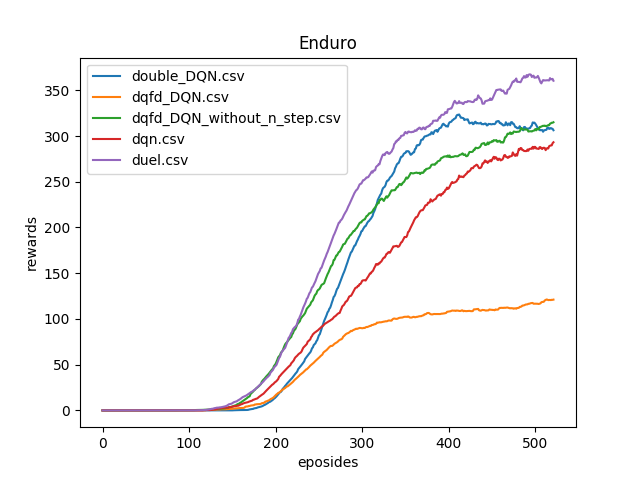
\includegraphics[scale=0.5]{../poster/figures/Enduro.png}
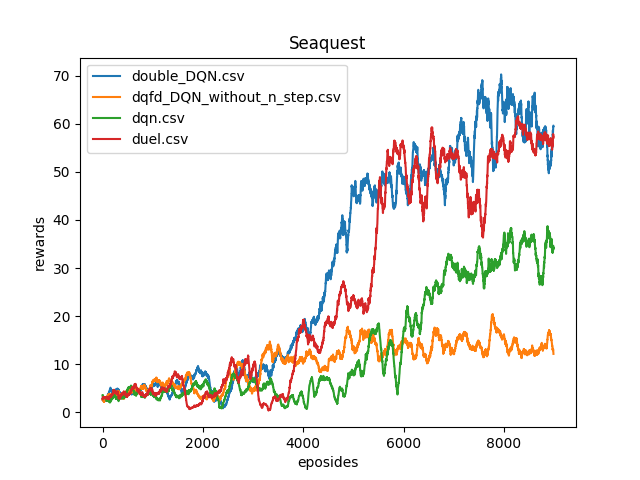
\includegraphics[scale=0.5]{../poster/figures/Seaquest.png}\\
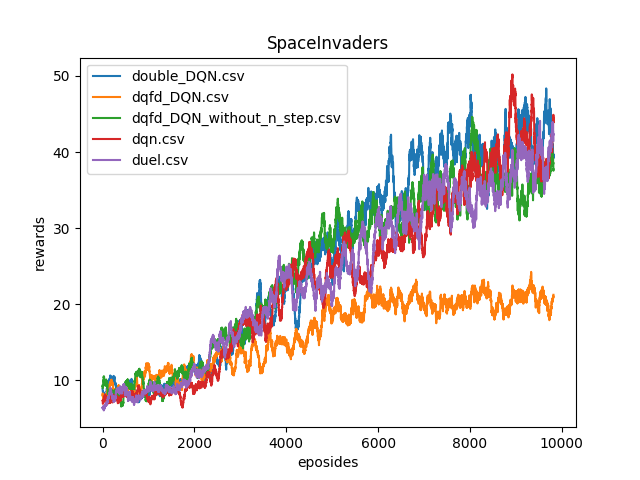
\includegraphics[scale=0.5]{../poster/figures/SpaceInvaders.png}

\caption{The learning curves of each model. Three games are used in out experiment, where Enduro is a racing game whose actions contains only ``left'', ``right'' and ``accelerate''; Seaquest and SpaceInvaders are both shooting games, in which Seaquest is more complicated. Our implementation of DQfD is on the basis of DDQN. In other words, the term $\mathcal{L}_{DQ}(w)$ in the DQfD loss function is same as the loss function of DDQN.}
\label{fig:results}
\end{figure}


Table~\ref{tab:dqn} denotes the network architecture. All models uses the left one except the Dueling DQN. We implemented these networks on \texttt{pytorch 0.3.0}. the optimizer is RMSProp, the learning rate is 0.0001, $\gamma$ is 0.99. The target network will duplicate its weight from online network every 1000 steps, while the online network will update every 4 steps. The size of replay buffer is 10000, and the batch size for sampling replay buffer data is 32.\par

As for DQfD, the pre-training steps is 350000, the probability of sampling demonstrated data is 0.3. We took 10 for calculating n-step loss, and if n-step loss is applied, $\lambda_n$ is 1. The weight of supervised loss $\lambda_E$ is 1, and the margin size ($k$) is 0.8.


\section{Results \& Discussion}



Figure~\ref{fig:results} shows the learning curves on different games. Apparently, the performances of DQfD is under our expectation. We made some analysis on why it didn't outperform other algorithms:
\begin{itemize}
    \item Compared to the original descriptions form the paper, we didn't implement the so-called ``Priortized Replay Buffer'' during sampling on replay memory. That is, the demonstrated data have not higher proirities to be sampled first, which makes the model harder to learn from the demonstrated data.
    \item Upon pre-training, the model is supposed to perform a non-zero score on each game, but our implementation doesn't. The main reason is that in our implementation, there exists a random exploration schedule from fully random to 5\%, which might cause the pre-trained results to be refreshed.
    \item Our implementation with n-step loss behaves strangely. There might be some implementation issues.
\end{itemize}
In conclusion, our implementation isn't successful this time. As for the future work, we can start from the possible causes above.







\renewcommand\refname{References}
\bibliographystyle{abbrv}
\bibliography{report}

\end{document}

